\chapter{Architecture logicielle}

Notre projet peut être découpé en plusieurs modules comme montré précédemment. L’architecture de notre logiciel va donc s’appuyer sur cette structure modulaire. Chaque module sera relié aux autres par une interface centrale recoupant les fonctionnalités de chaque module.

\section{Description des modules}

\subsection{Préparation des données}

Le module de préparation des données est divisé en trois parties représentées sur la figure 6.

\paragraph{}

\begin{mdframed}[frametitle={Figure 6 : Diagramme de classes de la partie préparation des données}, innerbottommargin=10]
\begin{center}
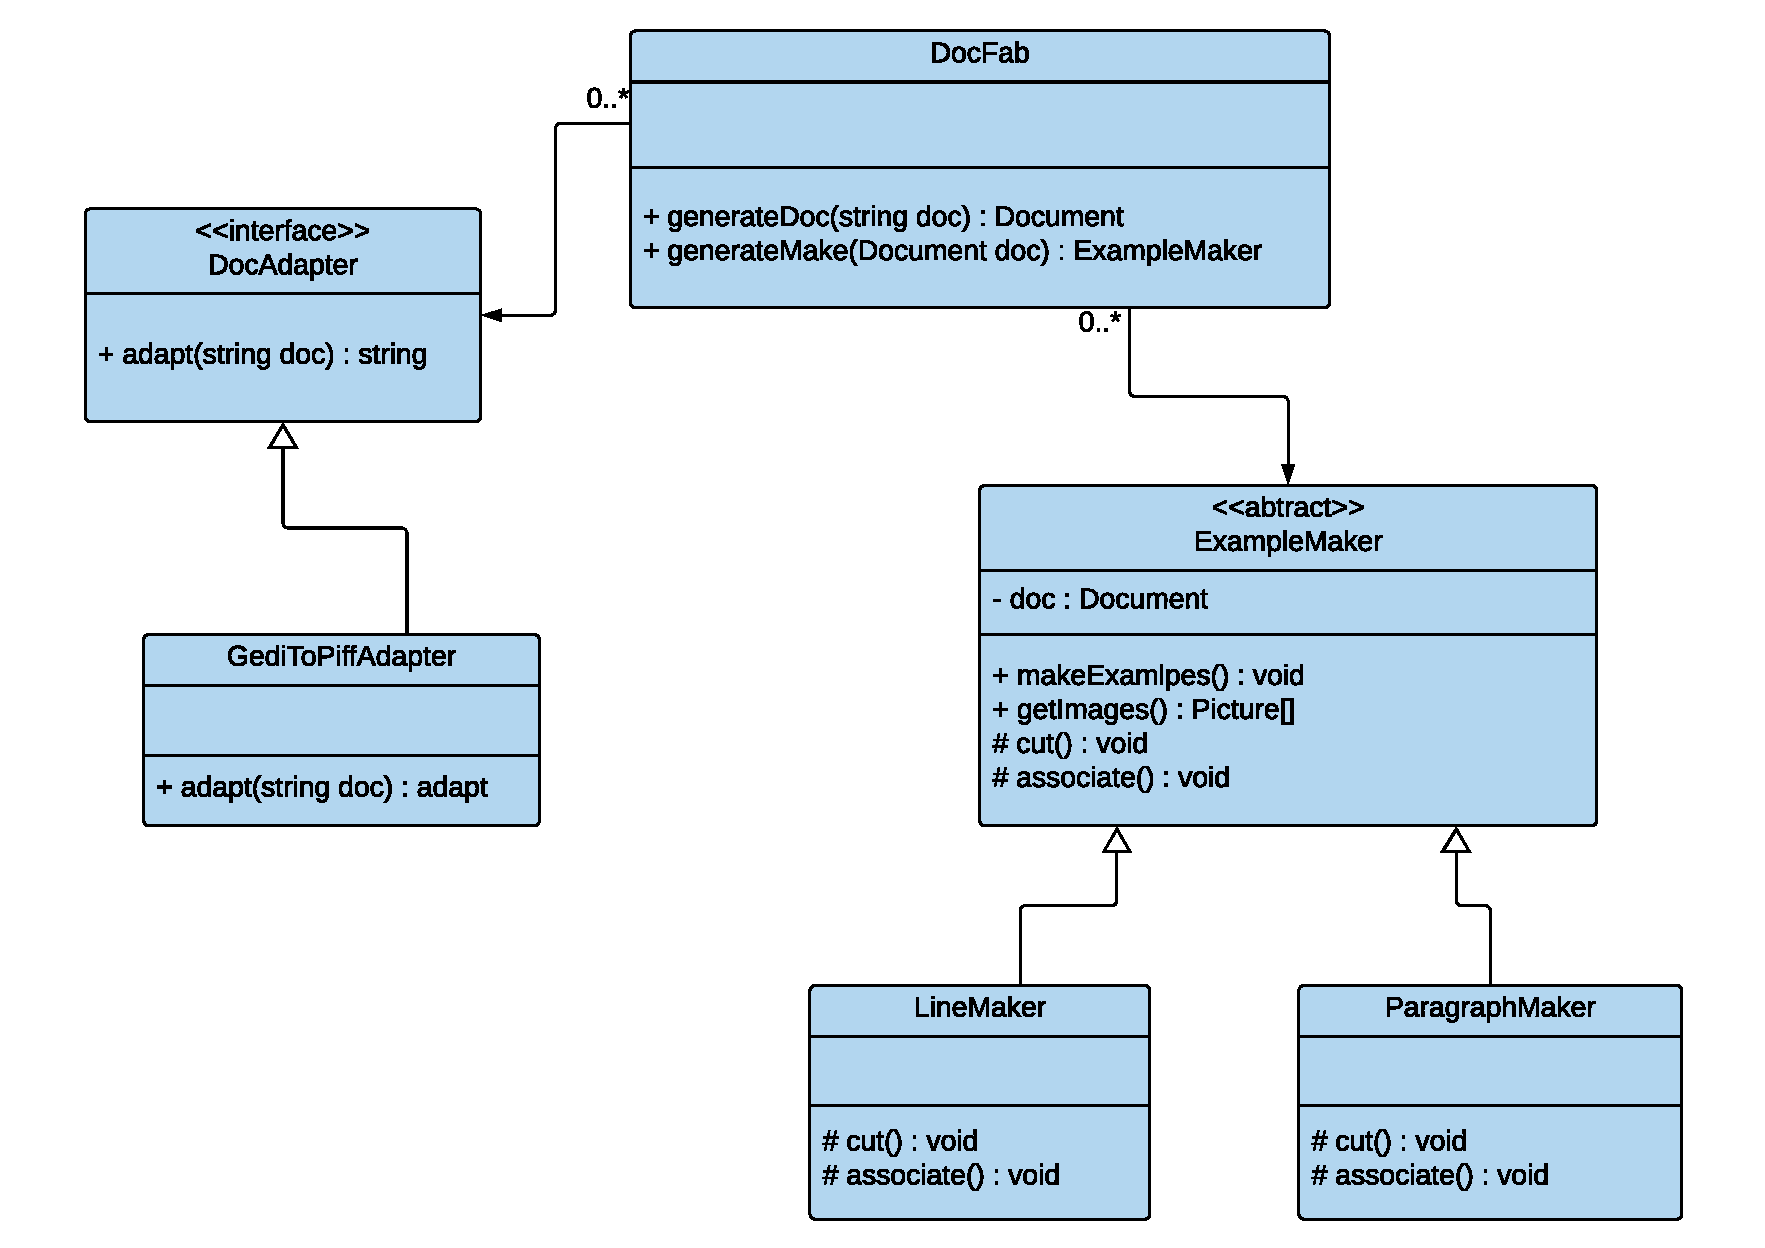
\includegraphics[scale=0.6]{prepa-data.pdf}
\end{center}
\end{mdframed}

\paragraph{}

La première est  une interface \textbf{DocAdapter} qui symbolise les convertisseurs de formats vers PiFF. Nous en implémenterons un, la classe \textbf{GEDIToPiFFAdapter}, afin de nous permettre de traiter comme prévu les documents de la base Maurdor, présentée dans le précédent rapport. Grâce à l’utilisation d’une interface, les développeurs sont cependant libres d’en ajouter à l’avenir.

\paragraph{}

La seconde partie est une classe abstraite \textbf{ExampleMaker} symbolisant la création des exemples d’apprentissage. En effet, les exemples peuvent être créés selon plusieurs méthodes de détection de lignes et de découpe d’images : par lignes ou par paragraphes. C’est pourquoi nous avons créé deux classes \textbf{LineMaker} et \textbf{ParagraphMaker}, mais une potentielle troisième méthode de détection de lignes à l’avenir pourra facilement être ajoutée à notre logiciel, en créant une troisième classe héritière d’\textbf{ExampleMaker}.

\paragraph{}

La troisième et dernière partie de ce module est une fabrique appelée \textbf{DocFab} sur la figure 6 qui utilise les deux parties présentées auparavant afin de créer des objets de type Document à partir d’une image et des données du fichier d’entrée.

\subsection{BDD}

Voici la manière dont nous avons modélisé la base de données :

\paragraph{}

\begin{mdframed}[frametitle={Figure 7 : Modèle entité association de la Base de données}, innerbottommargin=10]
\begin{center}
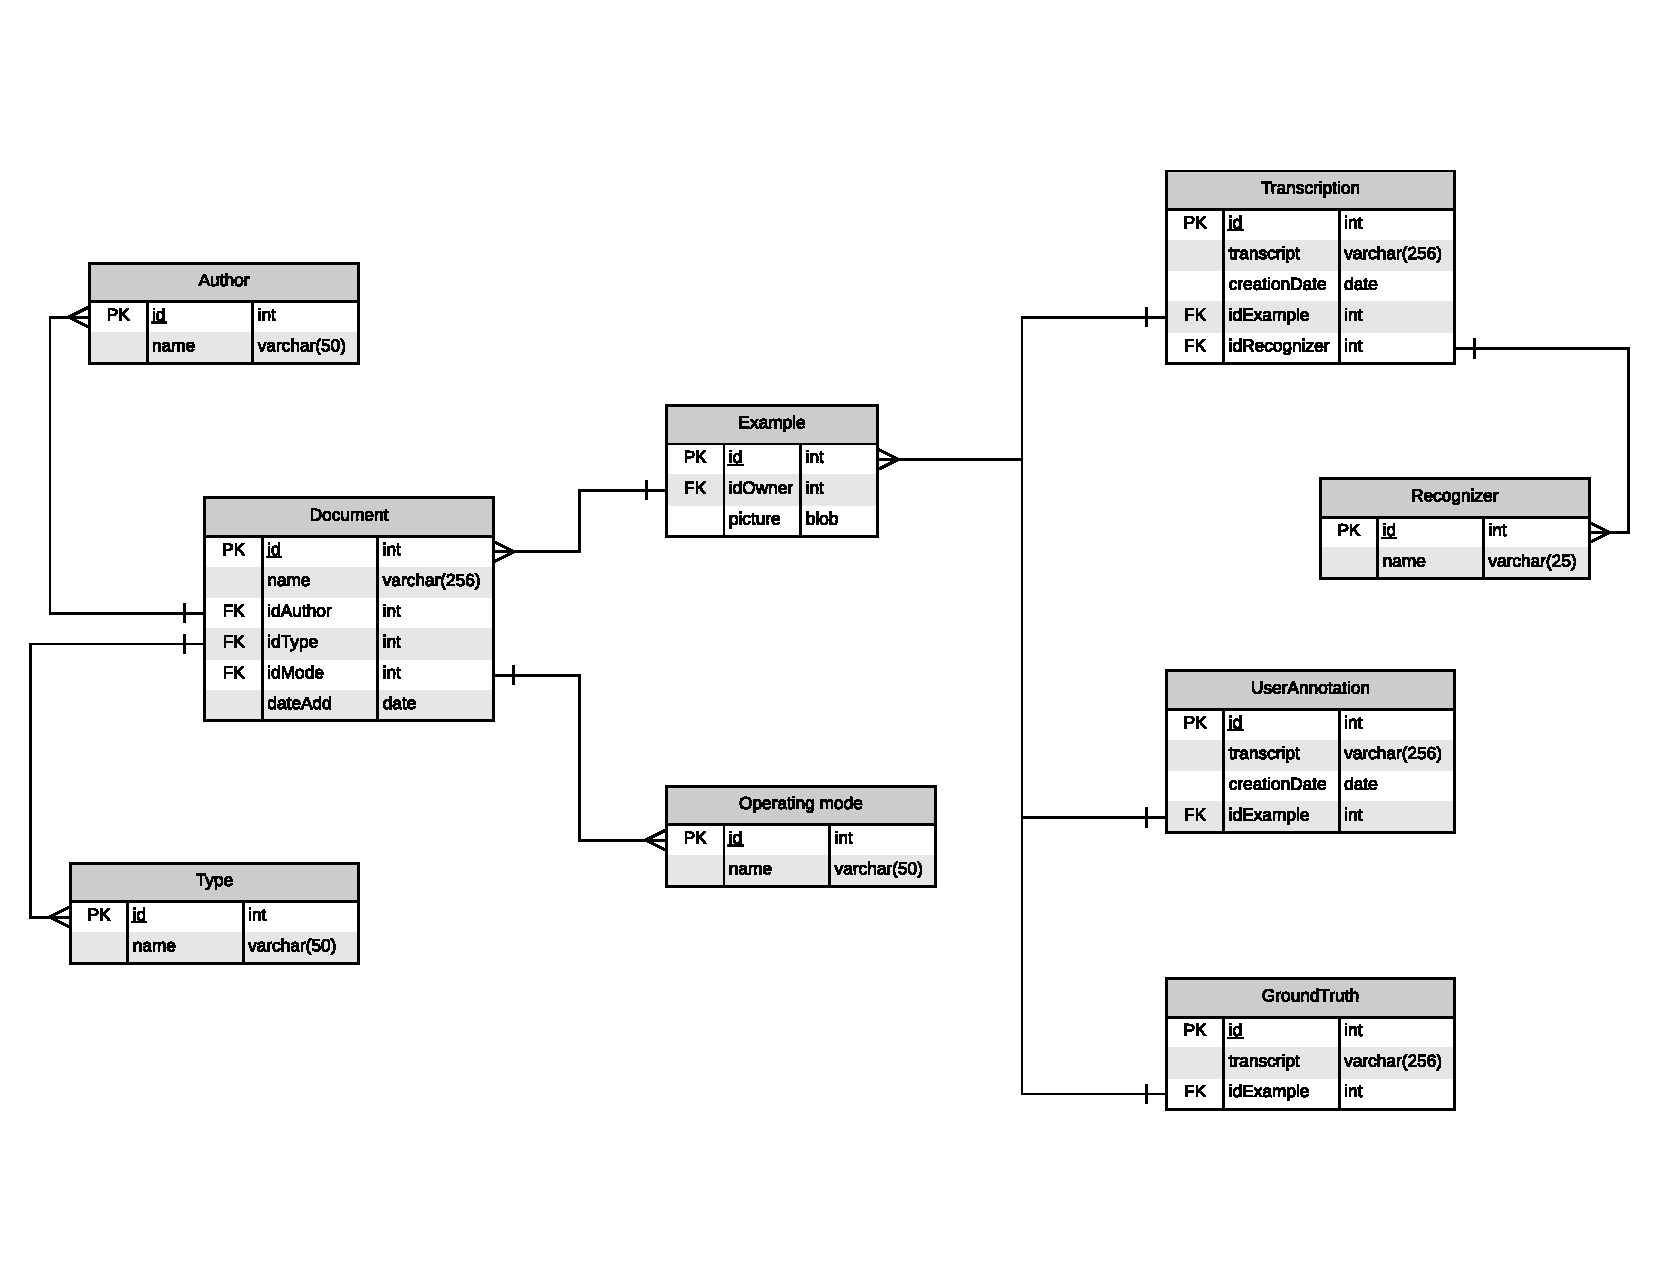
\includegraphics[scale=0.6]{Modele_entite_association.pdf}
\end{center}
\end{mdframed}

\paragraph{}

Les tables Author, Type et Operating Mode permettent de stocker les informations concerant les auteurs des documents, le type des documents ainsi que le mode dans lequel on se trouve (mode apprentissage ou mode évaluation).
La table Document contient toutes les informations concernant un document. A savoir son nom, son auteur, son type, le mode auquel il appartient ainsi que sa date d’ajout à la base.

Nos imagettes seront stockées dans des dossiers à côté de la base de données. Elles seront donc référencées par la base de donnée grâce à leur chemin (par exemple “/home/MesImagettes/imagette1.jpg”) dans la table Example. Cette table contient en plus une référence vers le document d’origine.

\paragraph{}

Les trois tables suivantes (Transcription, UserAnnotation, GroundTruth) servent à lier les imagettes avec leur transcription. Dans la table GroundTruth, on enregistre l’id de l’imagette ainsi que sa vérité-terrain. Dans la table UserAnnotation, on enregistre la même chose mais, en plus, la date de création de cette vérité-terrain qui aura été ajoutée par un utilisateur. Enfin, dans la table Transcription, on enregistre les mêmes informations que dans la table UserAnnotation sauf que, cette fois-ci, la transcription aura été donnée par un reconnaisseur d’écriture manuscrite représenté dans la table Recognizer.

\paragraph{}

La BDD sera gérée depuis le contrôleur via une classe Database contenant des méthodes pour communiquer avec elle. Une première version du diagramme de classes de cette partie est illustré en figure 7.

\paragraph{}

\begin{mdframed}[frametitle={Figure 8 : Diagramme de classes de l'interface avec la BDD}, innerbottommargin=10]
\begin{center}
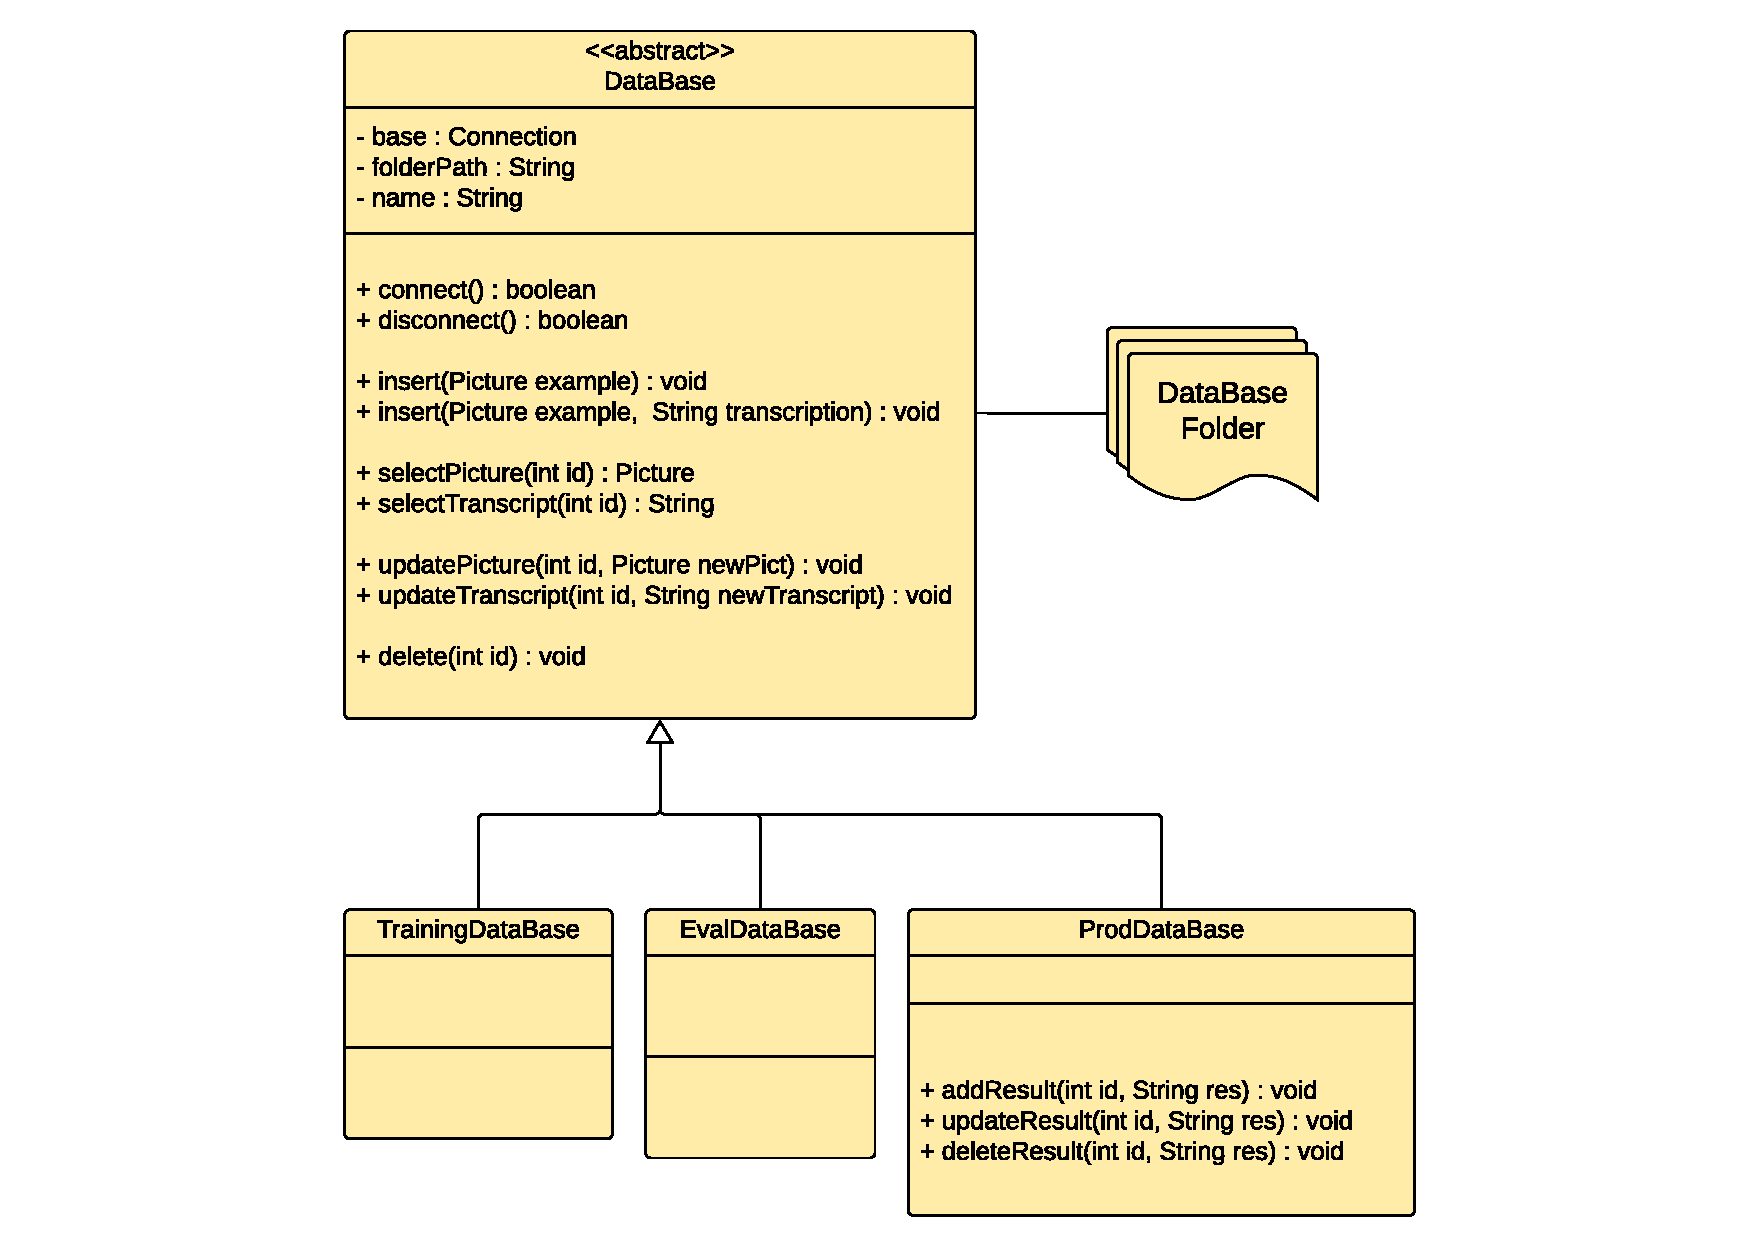
\includegraphics[scale=0.6]{bdd.pdf}
\end{center}
\end{mdframed}

\paragraph{}

Elle peut se connecter à la BDD et se déconnecter, ajouter des exemples avec et sans transcription, extraire des exemples et les modifier ou les supprimer. A chaque mode est associé une classe héritant de la classe \textbf{Database} et possédant les méthodes exclusives à ce mode. On obtient ainsi trois classes, \textbf{TrainingDataBase}, \textbf{EvalDataBase} et \textbf{ProdDataBase}, cette dernière classe pouvante également ajouter les résultats du classifieur.

\subsection{Interface avec le système de reconnaissance}

Le programme qui se chargera de faire l’interface entre les données de notre base et un reconnaisseur sera assez simple. Il se contentera d’extraire les données pertinentes de la base pour ensuite les convertir au bon format. Son architecture générale est illustrée pas le schéma ci-dessous.

\paragraph{}

\begin{mdframed}[frametitle={Figure 9 : Diagramme de classes de l'interface avec le système de reconaissance d'écriture manuscrite}, innerbottommargin=10]
\begin{center}
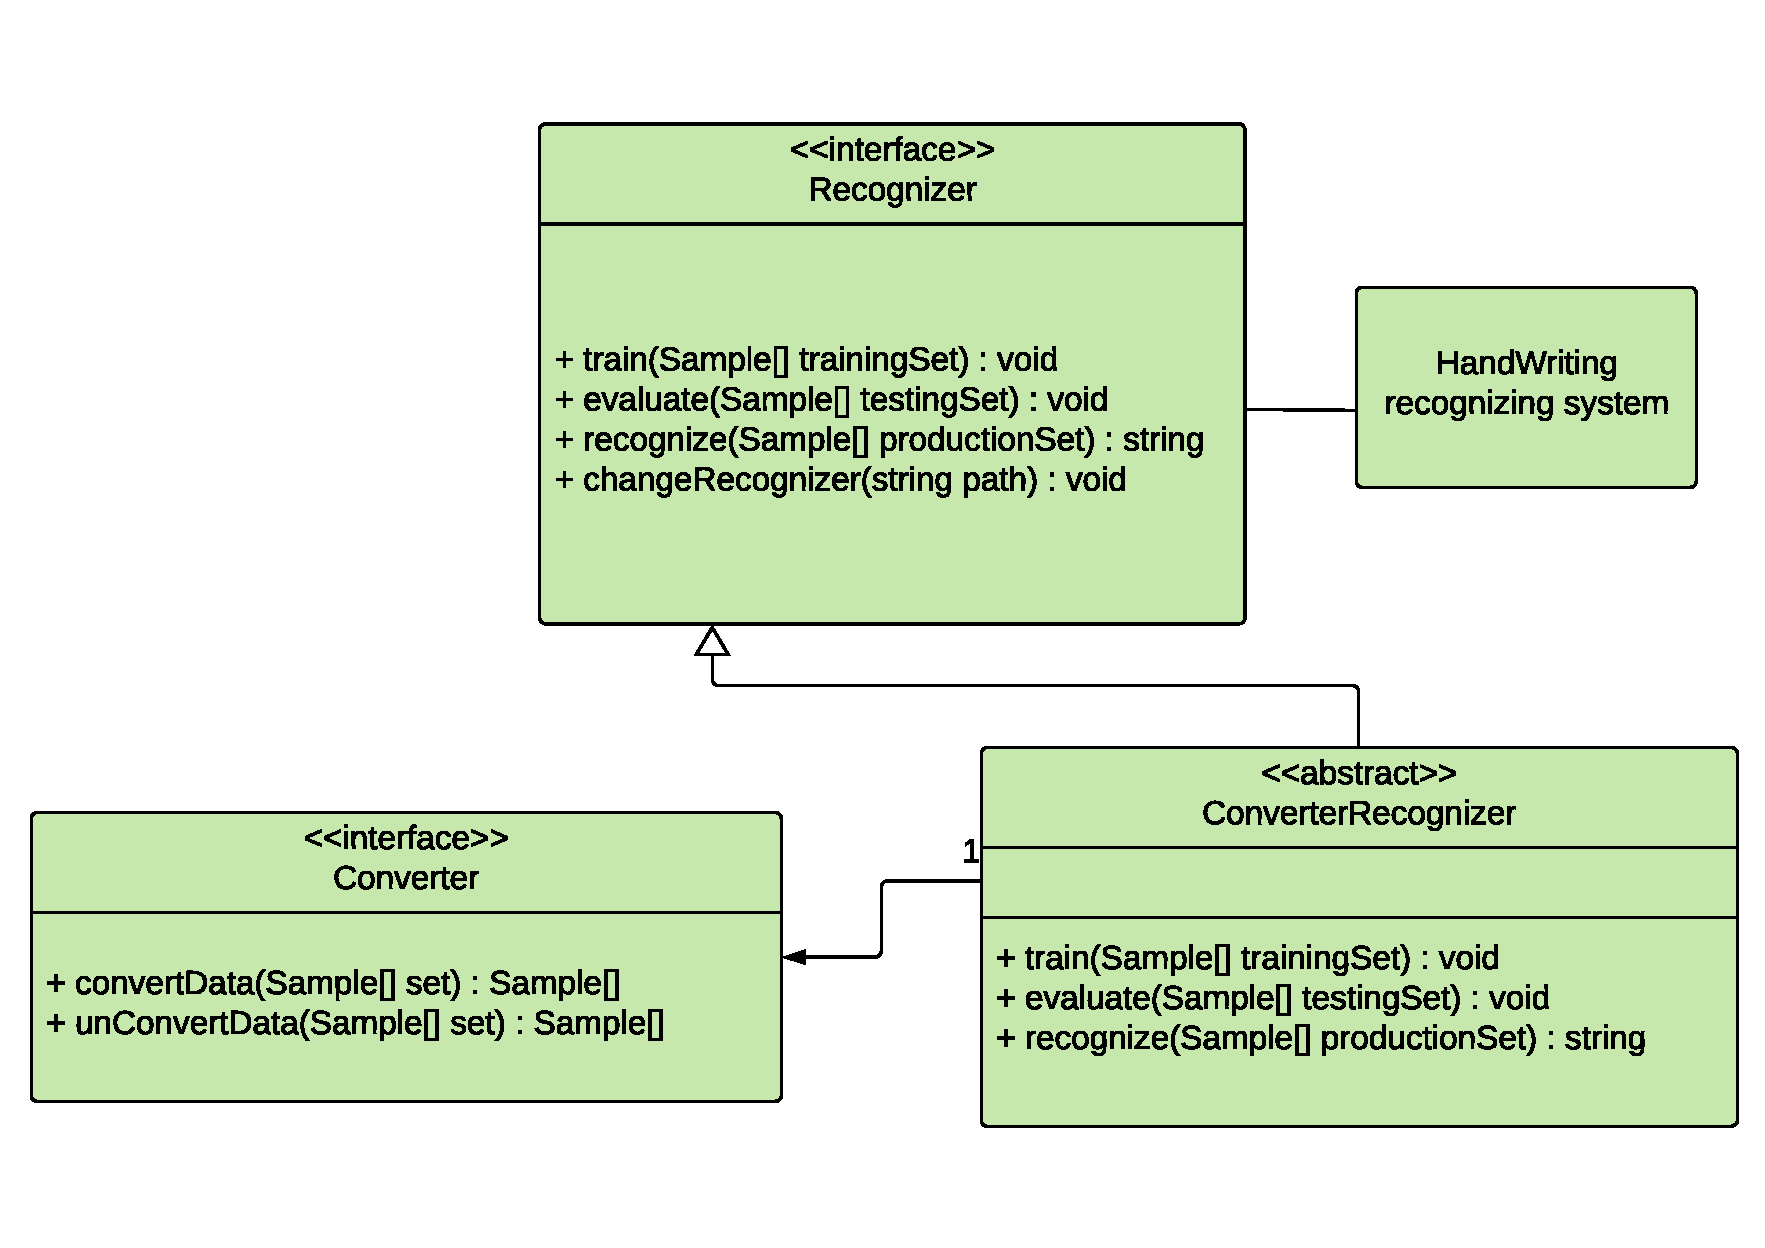
\includegraphics[scale=0.6]{interface-reconnaisseur.pdf}
\end{center}
\end{mdframed}

\paragraph{}

Une interface appelée \textbf{Recognizer} est associée au système de reconnaissance d’écriture manuscrite. cette interface possède des méthodes pour entraîner ou  évaluer le reconnaisseur, ou pour lui faire reconnaître des jeux de données. Un ensemble d’exemples est envoyé au reconnaisseur qui les traite.
Si les données nécessitent d’être converties, une classe \textbf{ConverterRecognizer} héritant de cette interface peut être utilisée. Elle possède en attribut une classe \textbf{Converter} pouvant exécuter des méthodes pour convertir les exemples d’un format à un autre. Ces méthodes de la classe Converter seront appelées par les méthodes d’entraînement, d’évaluation, … en amont du traitement qu’elles doivent effectuer.

\paragraph{}

Au cours du développement, des implémentations de ces interfaces ou classes abstraites seront réalisées.

\subsection{Interface Homme-Machine}

Le néant

\section{Interactions}

Tous les modules présentés dans la partie précédente doivent interagir entre eux à plusieurs niveaux. Un contrôleur général permet de gérer la communication et la coopération des différents modules. Une première architecture de celui-ci est visible sur la figure 10.

\paragraph{}

\begin{mdframed}[frametitle={Figure 10 : Diagramme de classes du contrôleur}, innerbottommargin=10]
\begin{center}
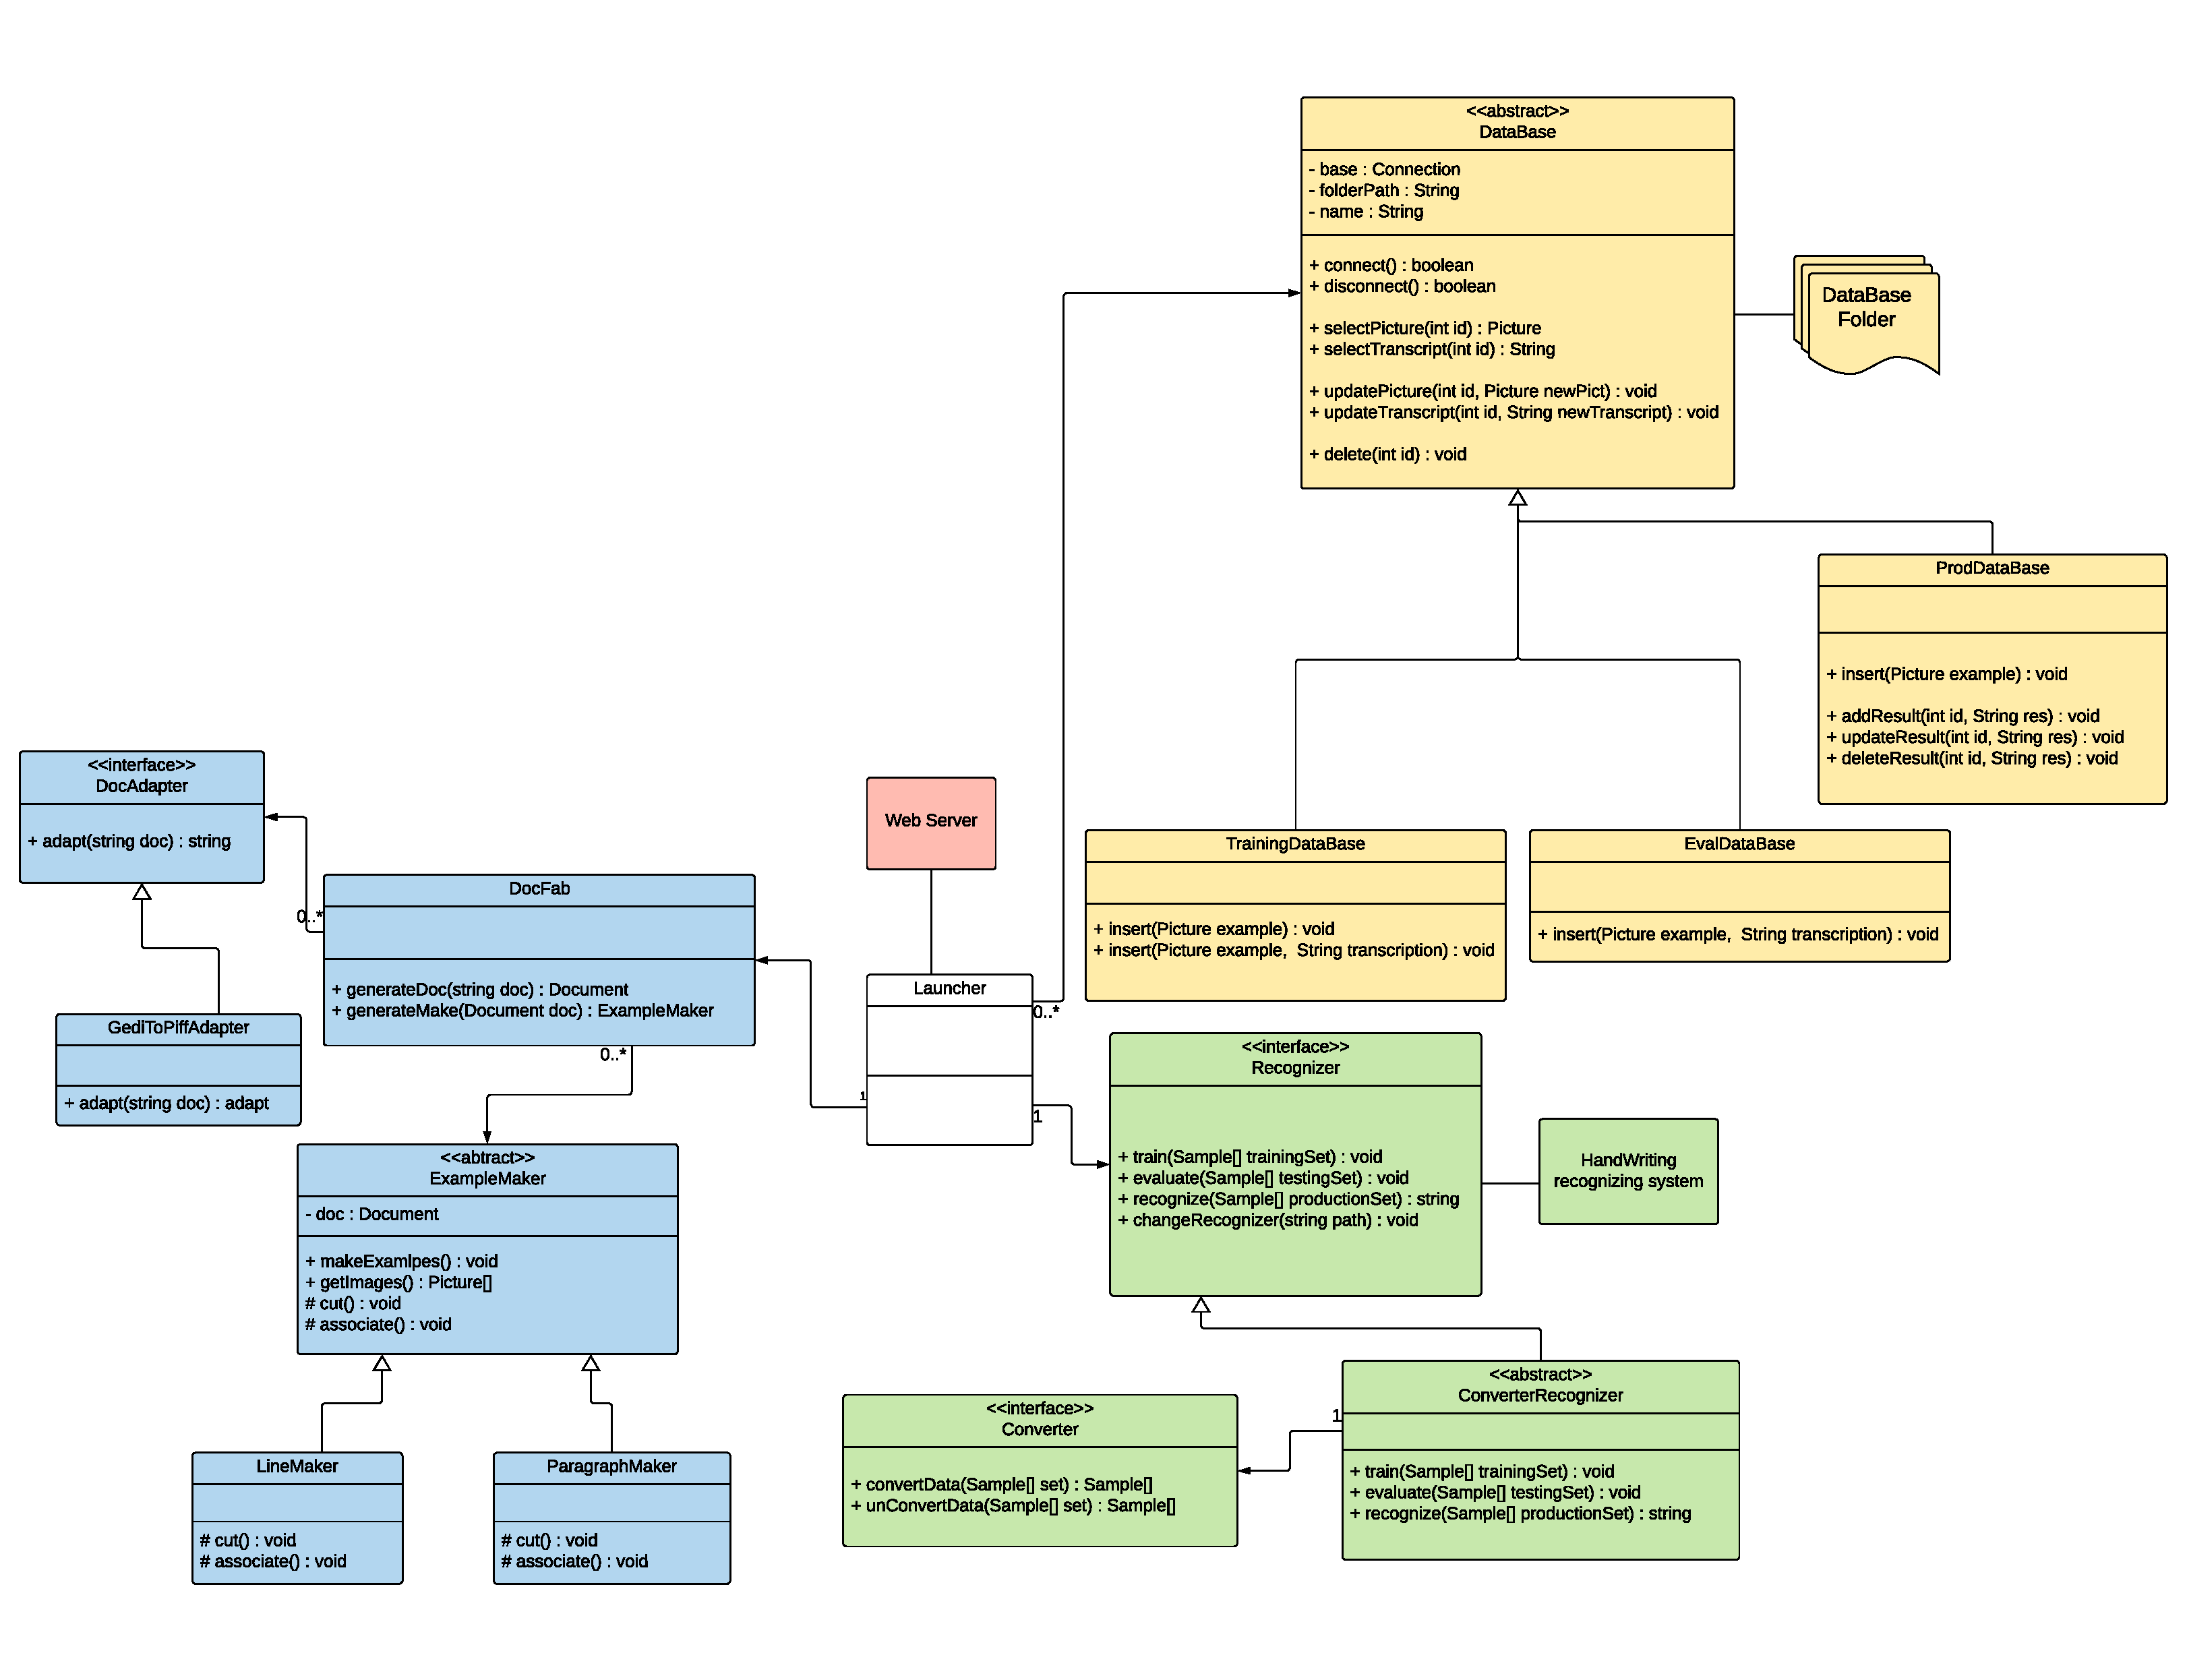
\includegraphics[scale=0.6]{Specifications.pdf}
\end{center}
\end{mdframed}

\paragraph{}

Le diagramme reste général et n’entre pas dans les détails de l’implémentation qui restent encore à définir. Les couleurs correspondant aux couleurs des parties expliquées sur la figure 1.

\paragraph{}

Le contrôleur possède une classe correspondant à la partie préparation des données (en bleu). Celle-ci contient des méthodes pour générer des exemples à ajouter à la BDD. Une autre classe (en jaune) permet de communiquer avec la BDD. Elle contient une méthode pour se connecter à la BDD, et d’autres pour envoyer, recevoir ou modifier des données stockées. Une dernière classe (partie en vert) permet ensuite de faire le lien avec le système de reconnaissance d’écriture manuscrite. Elle contient des méthodes pour lancer l’apprentissage ou l’évaluation du reconnaisseur ou pour l’utiliser sur un exemple en mode production.
Le contrôleur communique enfin avec l’IHM pour traiter les demandes de l’utilisateur et lui renvoyer les images et transcriptions. L’IHM est traitée par un serveur Web.


